\qrchapter{https://forgottenpillar.com/rsc/hr-fp-chapter3}{Povijesni Kontekst}

Ellen White se prisjetila susreta s istim sentimentima u \textit{Živom Hramu} protiv kojih je upozoravala na početku svoje službe:

\egw{Dok smo čitali \normaltext{[Živi Hram]}, prepoznala sam upravo one sentimente protiv kojih sam bila pozvana upozoravati \textbf{tijekom \underline{ranih dana} mojeg javnog djelovanja}. Kada sam prvi put napustila državu Maine, trebala sam proći Vermont i Massachusetts, kako bi svjedočila protiv tih sentimenata. \textbf{‘Živi Hram’ sadrži alfu tih teorija. Znala sam da će \underline{omega ubrzo uslijediti}; i drhtala sam za naš narod}. \textbf{Znala sam da moram upozoriti našu braću i sestre da ne ulaze u kontroverzu \underline{oko prisutnosti i ličnosti Boga}}. \textbf{Sentimenti u knjizi ‘Živi Hram’ \underline{vezani uz tu točku su netočni}}. Sveto Pismo koje se koristilo za potkrijepljenje te doktrine, je pogrešno primijenjeno.}[SpTB02 53.2; 1904][https://egwwritings.org/read?panels=p417.271]

Točno je odredila svoj prvi susret s tim pogledima: \egwinline{Kada sam prvi put napustila \textbf{državu Maine}, trebala sam proći Vermont i Massachusetts, \textbf{kako bi svjedočila protiv tih sentimenata}.} Njezina biografija, koju je napisao njezin unuk Arthur Lacey White, pruža dodatni kontekst o tim sentimentima. U \textit{Ellen White: Rane godine}, pod odjeljkom \textit{Borba s pogledima spiritualista}, njezina iskustva u istočnom Maineu otkrivaju više o kontroverzi oko ličnosti Boga i njezinim implikacijama.

\othersQuote{\textbf{\underline{U istočnom Maineu Ellen je putovala}} i radila \textbf{u atmosferi spiritualista koji su \underline{alegorijski poništili nebo, Boga, Isusa i adventnu nadu}}. U viđenju u Exeteru sredinom veljače činilo se da je \textbf{u Isusovoj prisutnosti, i bila je željna dobiti odgovore na neka \underline{vitalna pitanja}}.}[ALW, 1BIO 79.4; 1985][https://egwwritings.org/read?panels=p668.582]

\othersQuoteNoGap{Pitala sam Isusa \textbf{ima li Njegov Otac oblik poput Njega}. \textbf{Rekao je da ima}, ali ga ja nisam mogla vidjeti, jer je rekao: ‘Kad bi samo jednom ugledala slavu \textbf{Njegove osobe}, prestala bi postojati.’—Rani spisi, 54.}[ALW, 1BIO 79.5; 1985][https://egwwritings.org/read?panels=p668.583]

\othersQuoteNoGap{Ovo nije bila jedina prilika kada je Ellen razgovarala s Isusom i anđelom \textbf{o \underline{Isusovoj osobi} i o tome da je \underline{Bog osobno biće}}. \textbf{\underline{Odgovori su je potpuno uvjerili da su spiritualisti u velikoj zabludi}}.}[ALW, 1BIO 80.1; 1985][https://egwwritings.org/read?panels=p668.586]

Viđenje na koje se Arthur Lacey White referirao poznato je kao \textit{viđenje o ličnosti Boga}, koje ćemo kasnije razmotriti. Ovo viđenje potvrđuje da doktrina o \emcap{ličnosti Boga} uči da Bog Otac ima oblik, baš kao i Isus. Posebno se bavi \others{\textbf{Isusovom osobom} i time da je \textbf{Bog osobno biće}.}

Razmotrite prvu točku \emcap{Fundamentalnih principa}, koja navodi da Adventisti sedmoga dana vjeruju da \others{postoji jedan Bog, \textbf{osobno, duhovno biće}.}[Prva točka Fundamentalnih principa][https://forgotten-pillar.s3.us-east-2.amazonaws.com/A+declaration+of+the+fundamental+principles+taught+and+practiced+by+the+Seventh-day+Adventists++.pdf] Ovo jasno pokazuje da se središnje pitanje u doktrini o \emcap{ličnosti Boga} tiče vanjskog, tjelesnog oblika Oca. Ali zašto je to bilo tako vitalno i značajno pitanje? Koje su bile implikacije toga da Bog ima tjelesni, osobni oblik?

\begin{figure}[t]
    \centering
    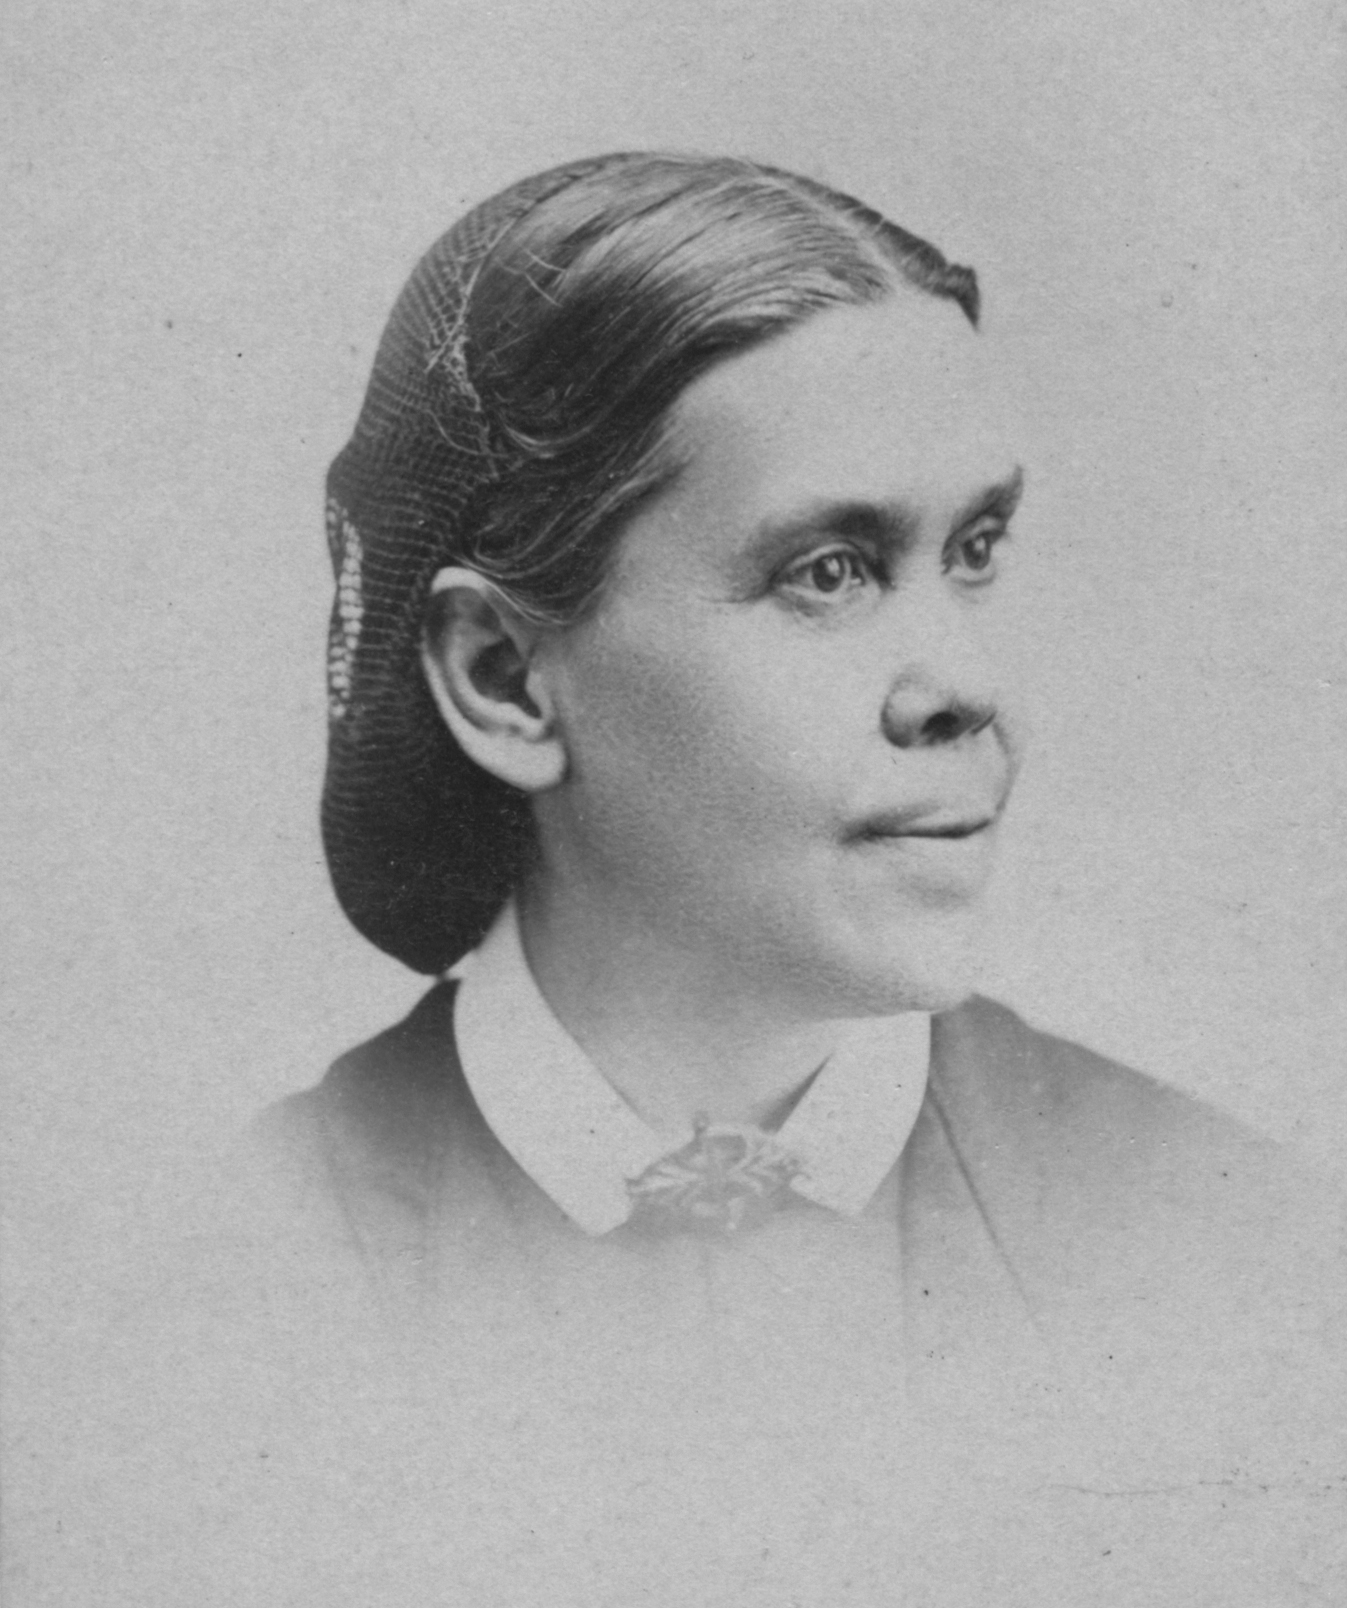
\includegraphics[width=0.65\linewidth]{images/ellen-white.jpg}
    \caption*{Ellen G. White}
    \label{fig:ellen-g-white}
\end{figure}

\othersQuote{Ali budući da su pioniri Crkve Adventista Sedmoga Dana smatrali da se proročanstvo ispunilo 22. listopada 1844., i da je važan rad započeo na nebu u Svetinji nad svetinjama nebeskog svetišta u to vrijeme, i budući da su adventisti koji su postali \textbf{spiritualisti} zauzeli stav da je Krist došao u njihova srca 22. listopada 1844., i da je Njegovo kraljevstvo u njihovim srcima, osnivači crkve, a posebno Ellen White, bili su svrstani od strane svijeta općenito, kao i od onih koje su adventisti sedmog dana nazivali adventistima prvog dana, u istu skupinu. Ovdje je ponovno veliki neprijatelj bacio ljagu na istinito, uspoređujući ga s lažnim, krivotvorenim iskustvom.}[ALW, 1BIO 80.2; 1985][https://egwwritings.org/read?panels=p668.587]

\othersQuoteNoGap{Ellen White će ponovno govoriti o ovom pitanju, posebno u završnim odlomcima svoje prve male knjige, “Iskustva i Viđenja”, objavljene 1851. Dok čitamo ovo, primijetit ćemo uporabu \textbf{pojma spiritualizam}, koji se mora shvatiti u svjetlu rada spiritualista, a ne u svjetlu onoga što se danas podrazumijeva pod spiritualizmom ili spiritizmom, iako oboje potječu iz istog izvora.}[ALW, 1BIO 80.3; 1985][https://egwwritings.org/read?panels=p668.588]

\othersQuoteNoGap{Sada se okrećemo izjavi napisanoj i objavljenoj 1851. godine kako je zabilježeno u Ranim Spisima., 77, 78:}[ALW, 1BIO 80.4; 1985][https://egwwritings.org/read?panels=p668.589]

\othersQuoteNoGap{\textbf{Često sam lažno optužena da naučavam gledišta svojstvena spiritualizmu}. Ali prije nego što je urednik The Day-Stara upao u tu zabludu, \textbf{Gospodin mi je \underline{dao viđenje} o žalosnim i pustošećim učincima koje će on i drugi proizvesti na stado \underline{naučavanjem duhovnih pogleda}}.}[ALW, 1BIO 80.5; 1985][https://egwwritings.org/read?panels=p668.590]

\othersQuoteNoGap{Često sam vidjela dragog \textbf{Isusa, da je On osoba}. Pitala sam Ga \textbf{\underline{je li Njegov Otac osoba} i \underline{ima li oblik} poput Njega}. Isus je rekao: ‘Ja sam \textbf{savršena slika osobe Moga Oca}.}[ALW, 1BIO 80.6; 1985][https://egwwritings.org/read?panels=p668.591]

\othersQuoteNoGap{\textbf{Često sam vidjela da je \underline{duhovni pogled} oduzelo svu slavu neba, i da su u mnogim umovima Davidovo prijestolje i draga osoba Isusa izgorjeli u vatri spiritualizma.} Vidjela sam da će neki koji su bili prevareni i uvedeni u ovu zabludu biti izvedeni na svjetlo istine, ali će im biti gotovo nemoguće potpuno se osloboditi \textbf{varljive moći spiritualizma}. Takvi bi trebali temeljito priznati svoje zablude i zauvijek ih napustiti.}[ALW, 1BIO 80.7; 1985][https://egwwritings.org/read?panels=p668.592]

\othersQuoteNoGap{\textbf{Spiritualizacija neba, Boga, Krista i Kristovog dolaska bila je temelj mnogih fanatičnih učenja s kojima je 17-godišnja Ellen Harmon bila pozvana od Boga da se suoči u tim formativnim danima. Viđenja su čvrsto uspostavila \underline{ličnost Boga i Krista}, \underline{stvarnost neba} i nagradu vjernima, te uskrsnuće. Ovo zdravo vodstvo spasilo je crkvu u nastajanju}.}[ALW, 1BIO 81.1; 1985][https://egwwritings.org/read?panels=p668.595]

Pogreška mileritskog pokreta 1844. godine ležala je u pogrešnom razumijevanju prirode događaja, a ne njegovog vremena. Daniel 7:13-14 opisuje Krista kako dolazi Pradavnome na nebu da primi vlast, slavu i kraljevstvo, a ne Njegov drugi dolazak na zemlju. Ovaj događaj, koji označava početak Kristovog rada u Svetinji nad svetinjama, dogodio se na završetku proročanstva o 2300 dana 1844. godine. Za razliku od drugih adventističkih skupina, Crkva Adventista Sedmoga Dana u nastajanju jedinstveno je prepoznala ovaj nebeski događaj.

Ovo razumijevanje temelji se na ključnim pretpostavkama:
\begin{itemize}
    \item Nebo je stvarno, doslovno mjesto (Ivan 14:1-3).
    \item Postoji doslovno svetište na nebu gdje Krist služi (Hebrejima 8:2).
    \item Postoji stvarno, fizičko prijestolje u tom svetištu, na kojem sjedi sâm Bog (Daniel 7:9-10; Otkrivenje 4:2-3; Ezekiel 1:26-28; Psalam 11:4).
\end{itemize}

Zašto je pitanje Očevog tjelesnog oblika tako važno? Kad Bog ne bi bio fizičko biće, ne bi bilo potrebe za doslovnim prijestoljem, svetištem ili nebeskom službom. Duhovna interpretacija potkopava temelj adventističke teologije, dovodeći do domino efekta koji u konačnici narušava doktrinu Kristove svećeničke službe.

Doktrina o \emcap{ličnosti Boga} bila je jednostavno ali temeljno učenje, potvrđeno u prvoj točki \emcap{Fundamentalnih Principa}: \textit{“Jedan Bog, osobno, duhovno biće.”} Kao takav, On nije sveprisutan sam po sebi već kroz svojega predstavnika, Svetog Duha.\footnote{Prva točka Fundamentalnih Principa: \othersQuote{Da postoji \textbf{jedan Bog}, \textbf{\underline{osobno, duhovno biće}}, stvoritelj svega, svemoguć, … i \textbf{svugdje prisutan po \underline{svom predstavniku}, Svetome Duha}. Ps. 139:7.}} Kada je Ellen White pitala Isusa \egwinline{je li Njegov Otac \textbf{osoba} i \textbf{ima li \underline{oblik}} poput Njega,}[EW 77.1; 1882][https://egwwritings.org/read?panels=p28.490&index=0] jasno vidimo da je \textit{vanjski tjelesni \textbf{oblik}} \textit{kvaliteta ili stanje koja nekog čine osobom}. Ovo razumijevanje bilo je ključno u rješavanju Kelloggove krize vezane uz \textit{Živi Hram}, koji je odstupao od ovog temeljnog vjerovanja.

Ali potvrđuju li naša trenutna \textit{Temeljna Vjerovanja} još uvijek ovu doktrinu? Poučavaju li izričito da je Bog stvarna osoba s tjelesnim oblikom, čija je doslovna prisutnost na nebu, dok je sveprisutan kroz svojeg Duha? Doktrina o Božjoj prisutnosti i ličnosti odsutna je iz današnjih službenih vjerovanja. Iako pojedinačno možda još uvijek vjerujemo u to, zašto je takvo vitalno učenje izostavljeno? Koji su bili razlozi za ovu promjenu? To su pitanja koja moramo dalje istražiti u kontekstu \textit{Temelja Naše Vjere}.

% The Historical Context

\begin{titledpoem}
    \stanza{
        U ranim danima svog djelovanja, \\
        Ellen je stala protiv krivog tumačenja. \\
        Upozorila je na alfu zabluda tih, \\
        Drhtala je znajući da omega slijedi njih.
    }

    \stanza{
        Bog ima oblik, to vizija otkriva, \\
        Kao što i Isus u obliku prebiva. \\
        Spiritualisti su nebo poništili, \\
        Božju ličnost lažno tumačili.
    }

    \stanza{
        Temelj vjere bio je jasan i čvrst, \\
        Bog je osoba, ne tek duh pust. \\
        Zašto je danas ta istina skrivena? \\
        Iz naših vjerovanja tiho uklonjena?
    }
\end{titledpoem}